%% Figure from MATH 556 notes, section 49 (Lecture 22). ADDED (not from lecture).
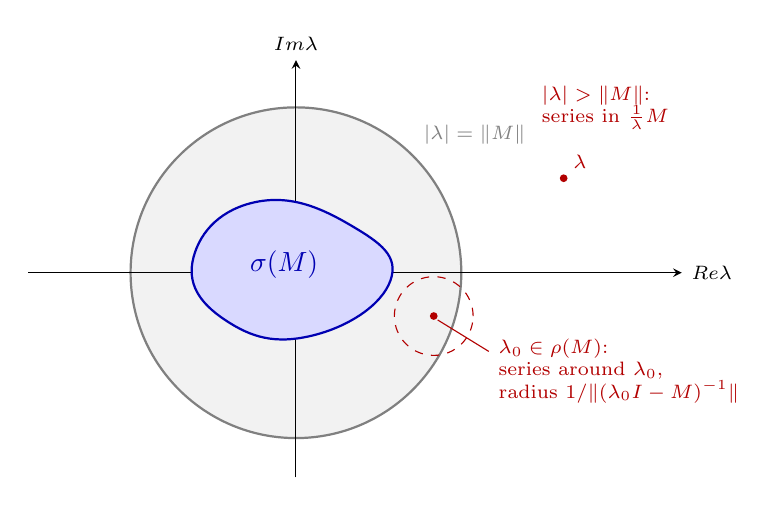
\begin{tikzpicture}[scale=1.0, >=stealth]
    \fill[gray!10] (0,0) circle (2.1);
    \draw[thick, gray] (0,0) circle (2.1);
    \draw[->] (-3.4,0) -- (4.9,0) node[right, font=\scriptsize] {$\operatorname{Re} \lambda$};
    \draw[->] (0,-2.6) -- (0,2.7) node[above, font=\scriptsize] {$\operatorname{Im} \lambda$};
    \draw[thick, blue!70!black, fill=blue!15] plot[smooth cycle, tension=0.8] coordinates {(-1.3,0.2) (-0.5,0.9) (0.7,0.6) (1.2,-0.1) (0.2,-0.8) (-0.9,-0.6)};
    \node[blue!70!black] at (-0.15,0.1) {$\sigma(M)$};
    \node[gray, font=\scriptsize, anchor=south west] at (1.5,1.5) {$|\lambda| = \|M\|$};
    \fill[red!70!black] (3.4,1.2) circle (1.4pt) node[above right, font=\scriptsize] {$\lambda$};
    \node[red!70!black, font=\scriptsize, align=left, anchor=west] at (3.0,2.1) {$|\lambda| > \|M\|$:\\series in $\frac{1}{\lambda} M$};
    \fill[red!70!black] (1.75,-0.55) circle (1.4pt);
    \draw[dashed, red!70!black] (1.75,-0.55) circle (0.5);
    \draw[thin, red!70!black] (1.8,-0.6) -- (2.45,-1.0);
    \node[red!70!black, font=\scriptsize, align=left, anchor=west] at (2.45,-1.25) {$\lambda_0 \in \rho(M)$:\\series around $\lambda_0$,\\radius $1 / \|(\lambda_0 I - M)^{-1}\|$};
\end{tikzpicture}
